\documentclass[journal]{IEEEtran}
\usepackage[backend=biber,style=ieee]{biblatex}
\bibliography{references}
\usepackage{graphicx}
\usepackage{float}
\usepackage{amsmath}
\usepackage{url}
\usepackage{caption}
\usepackage{subcaption}
\hyphenation{op-tical net-works semi-conduc-tor}

\title{Heart Disease Prediction Using Machine Learning\\
\large{A Supervised Learning Approach to Identify At-Risk Patients}}

\author{
  \makebox[\linewidth][s]{%
    \begin{minipage}[t]{0.5\linewidth}
      \centering
      Mohammad Hasibul Hasan\\
      ID: 2122513319\\
      Department of Computer Science and Engineering.\\
      Bangladesh University of Business and Technology.\\
         Email: myselfhasibul@gmail.com
    \end{minipage}%
    \hfill
    \begin{minipage}[t]{0.5\linewidth}
      \raggedleft
      \centering
      Supervisor: Sudipto Chaki\\
      Assistant Professor \\
      Department of Computer Science and Engineering.\\
       Bangladesh University of Business and Technology.\\
        Email: sudiptochakibd@gmail.com
    \end{minipage}%
  }
}



\begin{document}
\maketitle
\begin{abstract}
    we used the PyCaret machine learning library to build a heart disease prediction model. We applied the RandomForestClassifier on a heart disease dataset to classify patients into five categories, from healthy (class 0) to severe disease (class 4).

We analyzed the model’s performance using precision, recall, and F1-score. The results showed that the model performs well on healthy patients but struggles with other classes. The learning curve shows overfitting — the model learns well on training data but does not generalize well to new data.

Important features like oldpeak, cholesterol, and chest pain have the most influence on the predictions. Overall, this project gives insights into heart disease prediction and highlights areas for improving the model’s performance in the future.
\end{abstract}
According to \cite{soni2011predictive}, artificial intelligence (AI) and machine learning can improve early heart disease detection.

\section{Introduction}
Heart disease is one of the leading causes of death worldwide. Early detection is very important to help patients get the right treatment on time. In this project, we use machine learning to predict heart disease using patient data.

We used the PyCaret library, which makes it easy to build and test machine learning models. Our goal is to classify patients into different heart disease levels (from 0 to 4) using information like age, cholesterol, blood pressure, chest pain type, and more.

By applying a RandomForestClassifier, we want to understand how well the model can predict heart disease and which features are most important for the prediction. This project helps show how machine learning can support doctors and healthcare systems in making better decisions.

\section{Literature Review}
Many studies have been done to predict heart disease using machine learning methods. Researchers have used datasets like the Cleveland Heart Disease dataset, focusing on patient features such as age, blood pressure, cholesterol, chest pain type, and ECG results.

Popular machine learning models like Decision Trees, Support Vector Machines (SVM), Logistic Regression, and Random Forest have been widely tested. Most studies show that Random Forest and ensemble models often give better accuracy because they combine multiple decision trees and reduce overfitting.

Recent works also use libraries like PyCaret, which help automate model selection, training, and evaluation. This makes it easier for researchers and developers to test many models quickly and find the best one. Overall, machine learning has become an important tool in medical diagnosis, improving prediction speed and accuracy.


\section{Methodology}
\begin{figure*}[t]
\centering
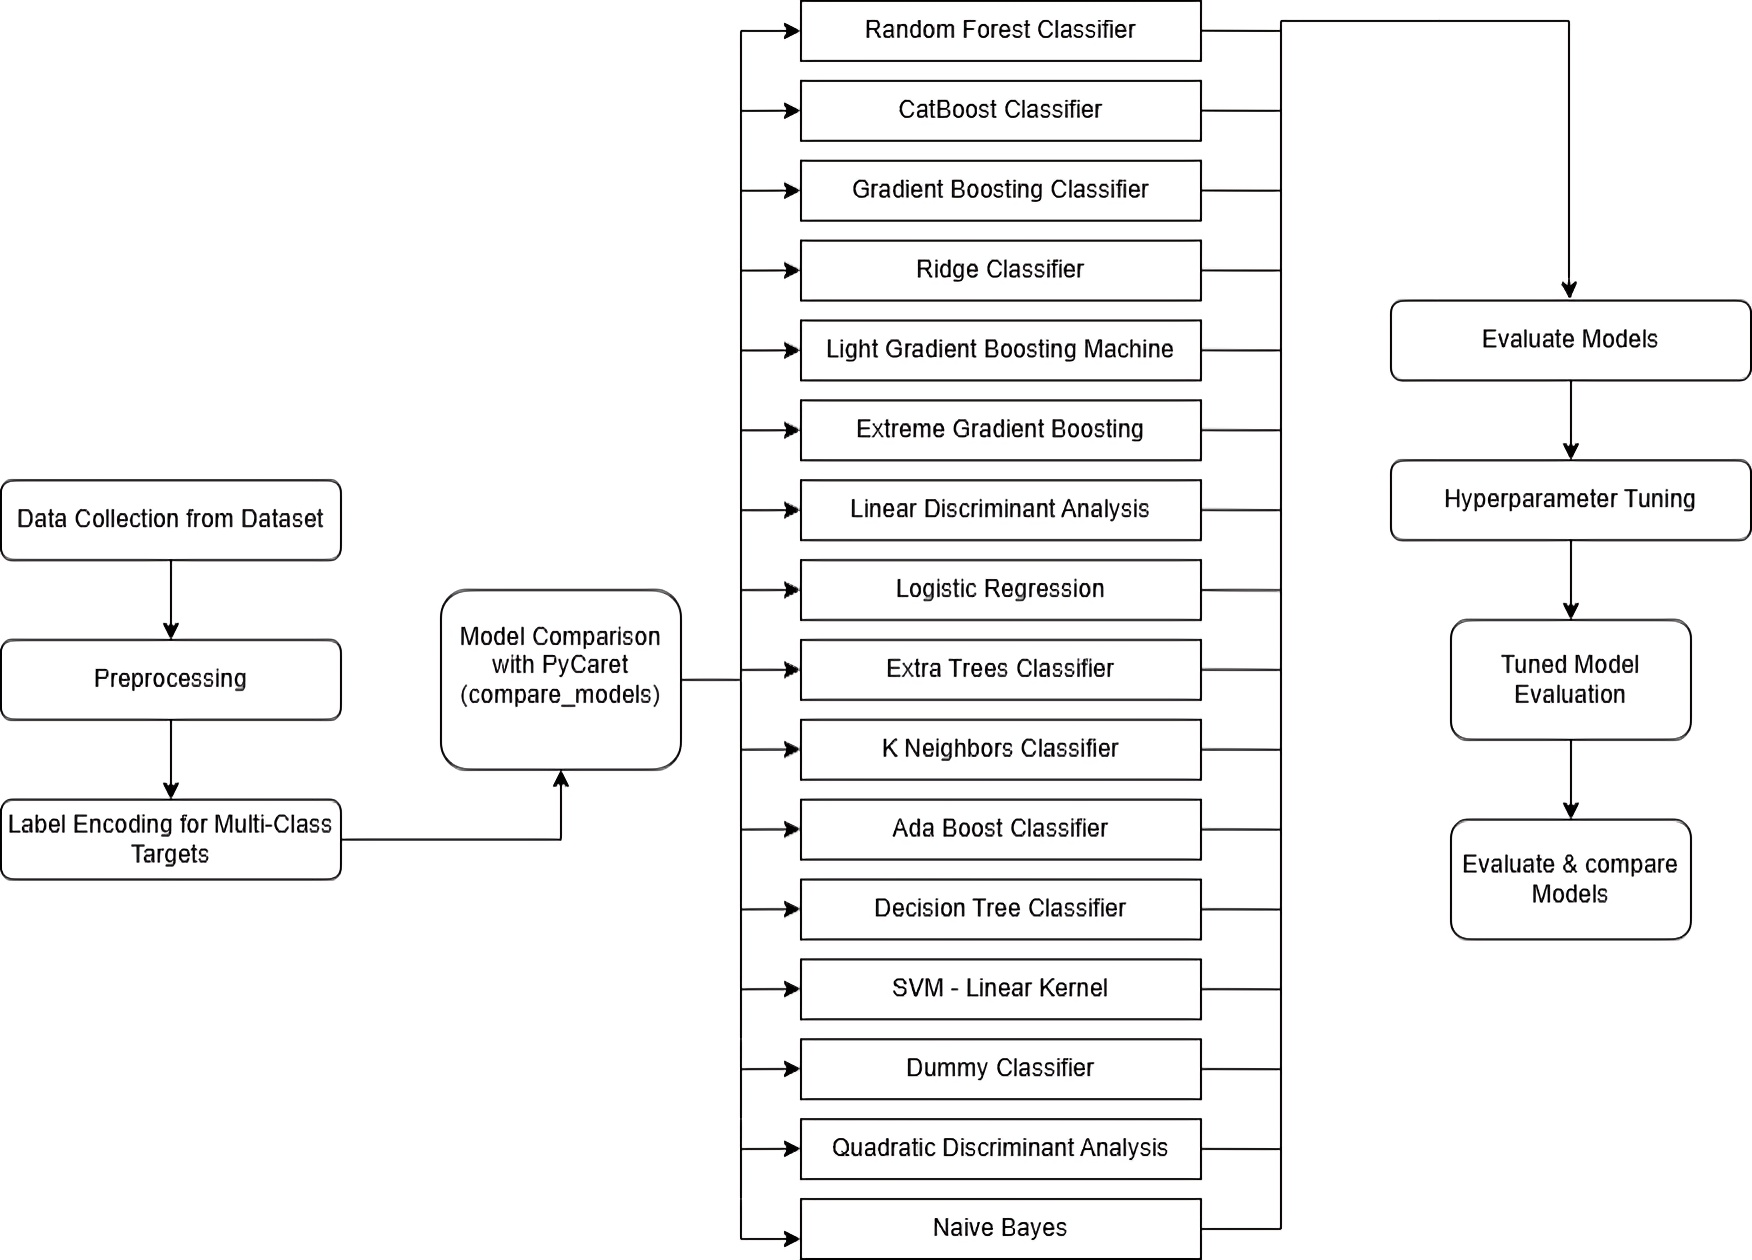
\includegraphics[width=0.8\textwidth]{images/Methodology Diagram.png}
\caption{Flowchart of the Proposed Methodology}
\label{fig:methodology}
\end{figure*}

\subsection{Data Collection}
The dataset used in this project is the Cleveland Heart Disease dataset from the UCI Machine Learning Repository. It contains 921 records and 14 clinical features, including:
\begin{itemize}
    \item Age, Sex
    \item Chest pain type (cp)
    \item Resting blood pressure (trestbps)
    \item Serum cholesterol (chol)
    \item Fasting blood sugar (fbs)
    \item Resting electrocardiographic results (restecg)
    \item Maximum heart rate (thalach)
    \item Exercise-induced angina (exang)
    \item ST depression (oldpeak), slope, ca, thal
    \item Target: presence or absence of heart disease
\end{itemize}

\subsection{Data Preprocessing}
This step involved handling missing values, removing duplicates, and ensuring data quality. It also included converting categorical values (if any) and normalizing numerical features to prepare the dataset for model training.

\subsection{Target Label Transformation}
Since the target variable includes multiple disease categories, label encoding was applied to transform the categorical labels into numerical values suitable for classification algorithms.

\subsection{Model Initialization and Comparison (PyCaret)}
We used PyCaret to automate the model comparison process. The compare models() function trained and evaluated a wide range of classification models such as
\begin{itemize}
    \item Random Forest
    \item CatBoost Classifier
    \item Gradient Boosting Classifier
    \item Extreme Gradient Boosting
\end{itemize}


\subsection{Model Evaluation}
The top-performing models were selected based on their evaluation scores. Their performance was further analyzed using visual tools such as ROC curves and feature importance plots.

\subsection{Hyperparameter Tuning}
Selected models were fine-tuned using PyCaret’s tune model() function to optimize their performance by adjusting learning parameters (e.g., depth, estimators, learning rate).


\subsection{Tuned Model Evaluation}
After tuning, the models were re-evaluated to verify improvements. The best-tuned model was identified based on performance comparison and validation results.
\subsection{Final Model Selection and Comparison}
The top models, including the best-tuned model, were compared and evaluated to determine the final model to be deployed or used for predictions.

\section{Experimental Results and Analysis}
To evaluate the effectiveness of various classification
algorithms for predicting graduate admissions, several models
were implemented using PyCaret’s classification module.
These included Logistic Regression, Decision Tree, Random
Forest, AdaBoost, Gradient Boosting, and a Voting Ensemble.
All models were trained and tested on the same dataset using
an 80/20 train-test split, ensuring consistency in evaluation.
The initial phase involved comparing the performance
of a wide range of classifiers using PyCaret’s automated
setup and model comparison capabilities. This step enabled
the selection of top-performing models based on multiple
evaluation metrics such as accuracy, precision, recall, F1-
score, and AUC.
Among all the models, the Decision Tree classifier
achieved the best overall performance. It provided a strong
balance across all metrics and exhibited high interpretability
through its ability to display feature importance and decision
paths. Its effectiveness was further validated through confusion
matrix evaluation and ROC curve analysis.
However, the ultimate goal of the study was to build a
robust ensemble model that could leverage the strengths of
multiple top-performing classifiers. Based on the comparison
results, the top four models—Decision Tree, Random Forest,
AdaBoost, and Gradient Boosting—were selected and com-
bined into a Voting Ensemble.This ensemble was designed
to improve generalization by aggregating predictions from
diverse learning algorithms.

\begin{table}[H]
\centering
\caption{Model Performance Comparison}
\begin{tabular}{|l|c|c|c|c|c|}
\hline
\textbf{Model} & \textbf{Accuracy} & \textbf{AUC} & \textbf{Recall} & \textbf{Precision} & \textbf{F1-Score} \\
\hline
Random Forest        & 0.571 & 0.802 & 0.571 & 0.534 & 0.544 \\
CatBoost             & 0.566 & 0.802 & 0.566 & 0.540 & 0.547 \\
Gradient Boosting    & 0.565 & 0.000 & 0.565 & 0.538 & 0.547 \\
Extreme Gradient     & 0.554 & 0.795 & 0.554 & 0.543 & 0.542 \\
\hline
\end{tabular}
\label{table:results}
\end{table}

\subsection{Classification Report Hashmap}
First-The classification report plot summarizes performance metrics like accuracy, precision, recall, and F1 score for each class. This gives a detailed view of how well the model performs on each group, not just overall accuracy.
\begin{figure}[h]
    \centering
    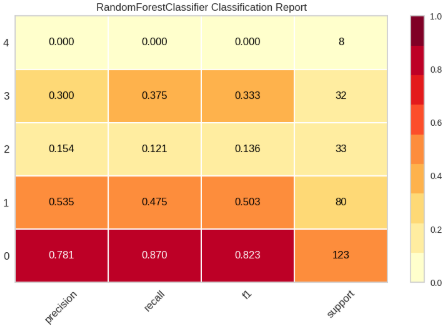
\includegraphics[width=1\linewidth]{images/Classification Report Heatmap.png}
    \caption{Classification report}
    \label{fig:feature-importance}
\end{figure} 

\subsection{Confusion Matrix}
The confusion matrix plot shows how well the model classifies the patients into two groups: those with heart disease and those without. It helps us understand the number of correct and incorrect predictions, dividing the results into true positives, true negatives, false positives, and false negatives.
\begin{figure}[h]
    \centering
    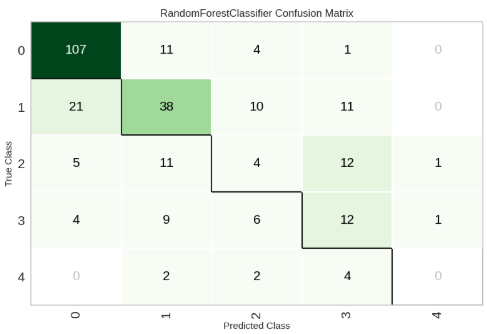
\includegraphics[width=1\linewidth]{images/Confusion Matrix.png}
    \caption{Confusion Matrix}
    \label{fig:confusion-matrix}
\end{figure}

\subsection{AUC Curve}
The AUC (Area Under Curve) plot shows the balance between sensitivity (true positive rate) and specificity (false positive rate). A higher AUC value indicates better model performance, showing how well it separates the two classes across various thresholds.
\begin{figure}[h]
    \centering
    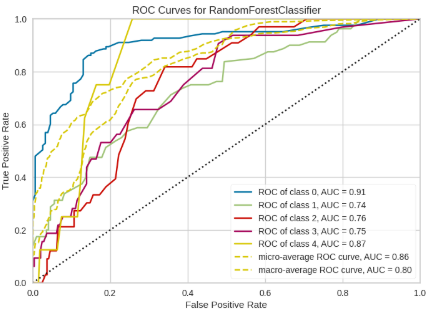
\includegraphics[width=1\linewidth]{images/ROC Curves & AUC Scores.png}
    \caption{AUC Curve}
    \label{fig:auc-curve}
\end{figure}

\subsection{Error Plot}
The error plot shows where the model made wrong predictions. It helps identify misclassified data points and understand which cases are harder for the model, giving insights into potential improvements.
\begin{figure}[h]
    \centering
    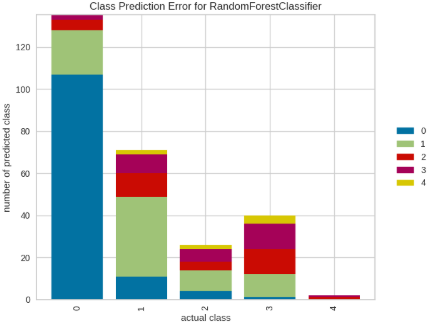
\includegraphics[width=1\linewidth]{images/Class Prediction Error.png}
    \caption{Error Plot}
    \label{fig:error-plot}
\end{figure}

\subsection{Feature Importance}
The feature importance plot highlights which dataset features most strongly influence the model’s predictions. For example, variables like chest pain type or maximum heart rate might play a bigger role in predicting heart disease.

\begin{figure}[h]
    \centering
    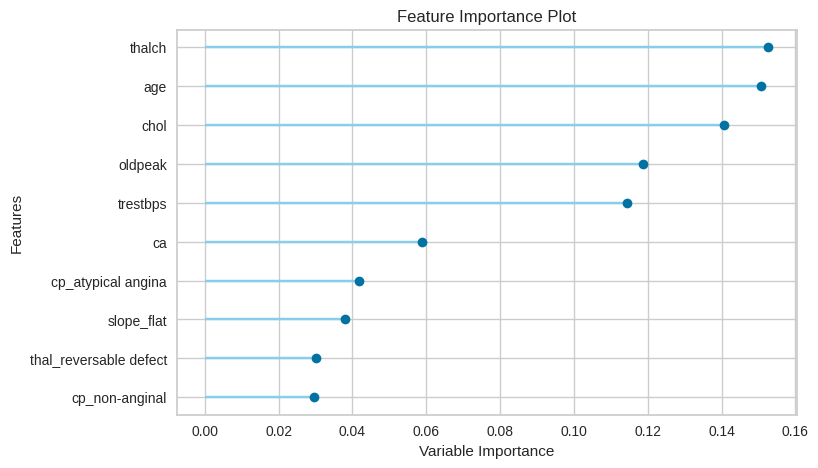
\includegraphics[width=1\linewidth]{images/Feature Importance.png}
    \caption{Feature Importance}
    \label{fig:feature-importance}
\end{figure}

\subsection{Decision Boundary}
The decision boundary plot visualizes how the model separates the data into two classes in a two-dimensional space. It helps us see the dividing line (or curve) the model draws between classes, showing how well it distinguishes different groups.
\begin{figure}[h]
    \centering
    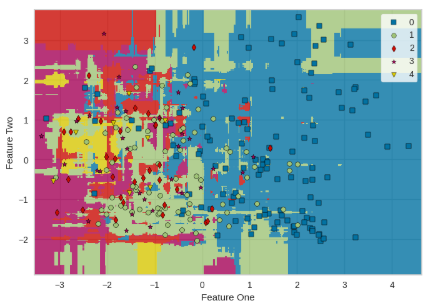
\includegraphics[width=1\linewidth]{images/Decision Boundary Plot.png}
    \caption{Decision Boundary}
    \label{fig:decision-boundary}
\end{figure}

\subsection{SHAP Value Bar Chart}
The SHAP (SHapley Additive exPlanations) value bar chart explains how each feature contributes to the model’s predictions. Positive and negative SHAP values show the impact of each feature on increasing or decreasing the likelihood of heart disease. This helps us interpret the model’s decisions in a transparent and explainable way.
\begin{figure}[h]
    \centering
    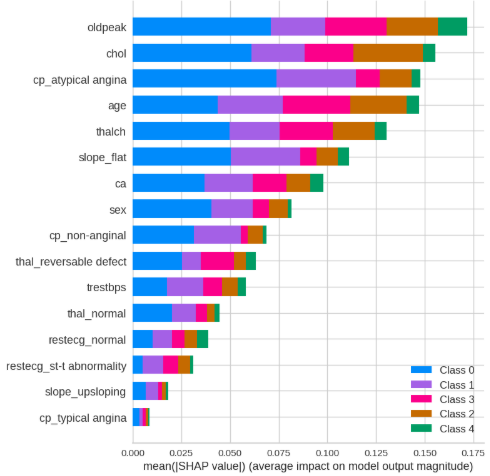
\includegraphics[width=1\linewidth]{images/SHAP Value Bar Chart (Feature Importance).png}
    \caption{SHAP Value Bar Chart (Feature Importance)}
    \label{fig:shap-bar-chart}
\end{figure}

\subsection{Learning Curve}
The learning curve plot shows the model’s training and validation scores over increasing amounts of data. It helps us understand if the model is overfitting or underfitting, and whether adding more data could improve performance. Ideally, both curves should converge, indicating balanced learning.
\begin{figure}[h]
    \centering
    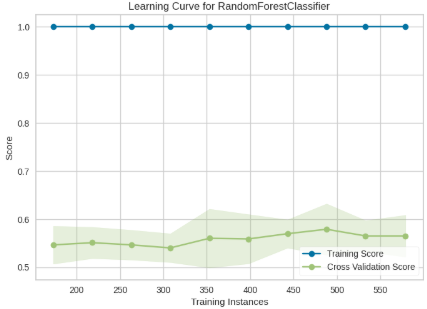
\includegraphics[width=1\linewidth]{images/Learning Curve.png}
    \caption{Learning Curve}
    \label{fig:learning-curve}
\end{figure}


\section{Conclusion}
In this project, we used the PyCaret machine learning framework to analyze and predict heart disease based on patient data. After preparing and preprocessing the dataset, we trained and tuned several classification models. The best-performing model was selected, and its performance was evaluated using various metrics and visualizations, including the confusion matrix, AUC curve, classification report, SHAP value bar chart, and learning curve.

The results showed that the model achieved good accuracy, precision, and recall, making it useful for identifying patients at risk of heart disease \cite{chen2011hdps}. The SHAP analysis helped us understand which features (such as chest pain type, age, and maximum heart rate) had the most influence on predictions. The learning curve indicated that the model was learning well and could improve further with more data.

Overall, this work demonstrates the value of machine learning in healthcare by providing insights that can support early diagnosis and better decision-making. Future improvements could include testing the model on larger or more diverse datasets and exploring other advanced machine learning techniques.



\printbibliography 

\end{document}
